Dette afsnit bygger på \cite{sandsynlighedsBog} og \cite{grimsandsynlighedsBog}
\begin{defn}
Lad $\{X_n\}_{n  \geq 0}$ være en følge af diskrete stokastiske variable med udfaldsrum $S$. Så kaldes $\{X_n\}_{n \geq 0}$ en diskret \textbf{Markov kæde}, hvis den overholder \textbf{Markov betingelsen}:
\begin{equation*}
    P(X_n = s \;| X_0 = x_0, \ldots, X_{n - 1} = x_{n - 1}) = P(X_n = s \;| X_{n - 1} = x_{n - 1})
\end{equation*}
for alle $n \in \N$ og $s, x_0, \ldots x_{n - 1} \in S$. Og i såfald kaldes $X_n$ \textbf{udfaldet} af Markov kæden i tiden $n$.
\end{defn}
\begin{exmp} Lad følgen af diskrete stokastiske variable $\{S_{n}\}_{n \geq 0}$, være definieret $S_{n} = \sum_{i=0}^n X_{i}$ for $n \in \N_{0}$, hvor $X_{i}$ er iid. diskrete stokastiske variable med $P(X_{i} = 1) = p$ og $P(X_{i} = -1) = 1 - p$. Så er $\{S_{n}\}_{n \geq 0}$ et eksempel på en Markov kæde \footnote{Faktisk er $\{S_{n}\}_{n \geq 0}$ et eksempel på hvad der kaldes en tilfældig tur}, da
  \begin{equation*}
    S_{n} = S_{n - 1} + X_{i} \implies P(S_{n} = k_{n} | S_{0} = k_{0}, \ldots, S_{n - 1} = k_{n - 1}) = P(S_{n} = k_{n} | S_{n - 1} = k_{n - 1})
  \end{equation*}
  for alle $k_{0}, k_{1}, \ldots, k_{n} \in \Z$.
\end{exmp}
\begin{defn}
Markov kæden $\{X_n\}_{n \geq 0}$ kaldes \textbf{homogen} hvis
\begin{equation*}
    P(X_n = i | X_{n - 1} = j) = P(X_1 = i | X_0 = j)
\end{equation*}
for alle $n \in \N$ og $i, j \in S$.
\end{defn}
Vi vil fremadrettet antage, at alle Markov kæder er homogene, medmindre andet eksplicit defineres.
\begin{defn}
Lad $\{X_n\}_{n \geq 0}$ være en Markov kæde, så defineres \textbf{overgangsmatricen} $P_X = [p_{ij}]$, hvor 
\begin{equation*}
    p_{ij} = P(X_1 = j \;| X_0 = i)
\end{equation*}
og \textbf{$n$ skridts overgangsmatricen} $P_X(n) = [p_{ij}(n)]$, hvor
\begin{equation*}
    p_{ij}(n) = P(X_n = j \;| X_0 = i)
\end{equation*}
\end{defn}

Det er ofte praktisk at visualisere Markov kæder som en vægtede og orienterede graf, hvor knudepunkterne repræsentere de forskellige udfald og kanterne imellem knudepunkt $i$ og $j$ er vægtet med $p_{ij}$. Bemærk, at kanten imellem $i$ og $j$ kun indtegnes i grafen, hvis $p_{ij} > 0$. Vi vil fremadrettet kalde sådanne en graf for \textbf{overgangsgrafen} af Markov kæden.
\begin{example}
  Betragt spillet roulette. Spillet består af 38 felter: 2 grønne, 18 røde samt 18 sorte. En kugle lander tilfældigt på et af felterne uafhængeligt af de tidligere runder. Der odses på hvilket type felt, den lander på. Vi vil i dette eksempel antage, at der odses, således at de grønne aldrig bliver valgt. Det koster $1\$$ at være med, men hvis kuglen lander på den korrekte farve, vinder man $2\$$. Det bemærkes, at den stokastiske process som er beskrevet her, opfylder Markov betingelsen, da hver runde er uafhængelige af hinanden. Det følger af beskrivelsen, at overgangsmatricen er givet som
  \begin{equation} \label{eq:transpositions_graf_roullete}
    P_{X} = \begin{bmatrix}
              1 & 0 & 0 & 0 & \ldots \\
              20 / 38 & 0 & 18 / 38 & 0 & \ldots \\
              0 & 20 / 38 & 0 & 18 / 38 & \ldots \\
              \vdots & \vdots & \vdots & \vdots & \ddots
            \end{bmatrix}
  \end{equation}
  Det mærkes, at da det koster $1 \$$ at spille, er $P(X_n = 0 | X_{n-1} = 0) = 1$. Udfra overgangsmatricen kan overgangsgrafen optegnes:
  \begin{figure}[H]
    \centering
    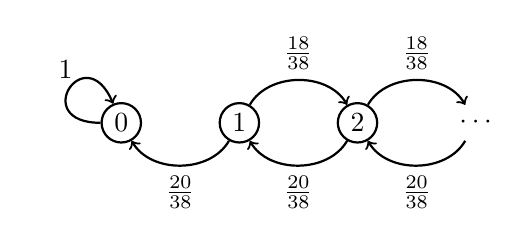
\begin{tikzpicture}
      \tikzset{punkt/.style={circle, thick, draw=black, minimum width=0.5cm,inner sep=0}}
      \node[punkt] at (-2.5, 0)      (a){$0$};
      \node[punkt] at (-1, 0)  (b){$1$};
      \node[punkt] at (0.5, 0)    (c){$2$};
      \tikzset{markus_m/.style={circle, thick, draw=white, minimum width=0.5cm,inner sep=0}}
      \node[markus_m] at (2, 0)    (d){$\cdots$};

      \draw[->, thick] (a) edge[out= 180, in = 113, looseness=8] node[above]{$1\;$} (a);
      \draw[->, thick] (b) edge[bend left=60] node[below]{$\frac{20}{38}$} (a);
      \draw[->, thick] (b) edge[bend left=60] node[above]{$\frac{18}{38}$} (c);
      \draw[->, thick] (c) edge[bend left=60] node[below]{$\frac{20}{38}$} (b);
      \draw[->, thick] (c) edge[bend left=60] node[above]{$\frac{18}{38}$} (d);
      \draw[->, thick] (d) edge[bend left=60] node[below]{$\frac{20}{38}$} (c);
    \end{tikzpicture}
    \caption{Overgangsgrafen for spillet roulette.}
    \label{fig:transpositions_graf_roullete}
  \end{figure}\noindent
  Bemærk, at ligesom, at vi har tale om en uendelig martix, har vi også tale om en overgangsgraf med uendeligt mange punkter.
\end{example}

Vi vil nu introducere følgende sætning, som giver os mulighed for at beregne $n$ skrids overgangsmatricer.
\begin{thm} \label{thm:n_skrids_transpositions_matrix}
Lad $\{X_n\}_{n \geq 0}$ være en Markov kæde, så er $P_X(n) = P_X^n$ for $n \in \N$.
\end{thm}
\begin{proof}
Vi beviser dette ved induktion. For $n = 1$ gælder ligheden per definition. Antag nu, at $P_X(n - 1) = P_X^{n - 1} = [p_{ij}(n - 1)]$, så er 
\begin{align*} 
    p_{ij}(n) = P(X_n = j \;| X_0 = i) &\stackrel{(a)}= \sum_{k \in S} P(X_n = j\; | X_{n - 1} = k, X_0 = i) P(X_{n - 1} = k\; | X_0 = i) \\
    &\stackrel{(b)}= \sum_{k \in S} P(X_n = j\; | X_{n - 1} = k) P(X_{n - 1} = k\; | X_0 = i) \\
    &= \sum_{k \in S} p_{jk}p_{ki}(n - 1) 
\end{align*}
Hvor lighed $(a)$ følger af sætning \ref{thm:LPT}, $(b)$ af Markov betingelsen. Men $\displaystyle \sum_{k \in S} p_{jk}p_{ki}(n - 1)$ er blot indgang $(i, j)$ i matrix produktet $P_X P_X(n - 1) = P_X P_X^{n - 1} = P_X^n$, per vores induktions antagelse.
\end{proof}

\begin{defn}
  Lad $\{X_{n}\}_{n \geq 0}$ være en Markov kæde, og lad $i \in S$:
  \begin{enumerate}[i)]
    \item Hvis $P(X_{n} = i \text{ for et } n \in \N \;| X_{0} = i) = 1$ kaldes $i$ \textbf{rekurrent}.
    \item Hvis $P(X_{1} = i \;| X_{0} = i) = 1$, så kaldes udfaldet $i$ for \textbf{absorberende}.
    \item Hivs $P(X_n = i \text{ for et } n \in \N \;| X_0 = i) < 1$ kaldes udfaldet \textbf{transient}
  \end{enumerate}
\end{defn}

\begin{remark}
  Det noteres, at ethvert absorberende udfald også er et eksmepel på et rekurrent udfald.
\end{remark}

\begin{example}
  Betragt igen spillet roulette og overgangsgrafen i figur \ref{fig:transpositions_graf_roullete} samt overgangsmatricen fra \ref{eq:transpositions_graf_roullete}. Det noteres, at udfaldet $0$ er et eksempel på et absorberende og rekurrent udfald, da $P(X_{1} = 0 | X_{0} = 0) = 1$. Derudover bemærkes det, at alle $i \in S \backslash \{0\}$ er eksempler på ikke rekurrente udfald, da $\exists n \in \N: P(X_{n} = 0 | X_{0} = i) > 0$. Tilgengæld er alle udfald $i \neq 0$ transiente, da $p_{ii}(2) = \sum_{j=0}^{\infty} p_{ij}p_{ji} > 0$, jævnfør sætning \ref{thm:n_skrids_transpositions_matrix}.
\end{example}

\begin{defn}
Lad $\{X_n\}_{n \geq 0}$ være en Markov kæde og $i, j \in S$. Udfaldene $i$ og $j$ siges, at \textbf{kommunikere}, skrevet $i \to j$, hvis $\exists m \in \N_0$, således $p_{ij}(m) > 0$. Hvis $i \to j$ og $j \to i$ siges $i$ og $j$ at \textbf{intrakommunikere}, skrives $i \leftrightarrow j$.\\ Lad $C \subseteq S$.
\begin{enumerate}[i)]
    \item Så kaldes $C$ \textbf{lukket} hvis $p_{ij} = 0$ for alle $i \in C, j \not \in C$. 
    \item og hvis  $i \leftrightarrow j$ for alle $i, j \in C$ kaldes $C$ \textbf{irreducibel}.
\end{enumerate}
\end{defn}

\begin{defn}
Lad $\{X_n\}_{n \geq 0}$ være en Markov kæde. En vektor $\bs{\pi}$, med indgange $\pi_j \in \R^+$ for $j \in S$, kaldes en \textbf{stationær fordeling} af $\{X_n\}_{n \geq 0}$, hvis $\bs{\pi}P_X = \bs{\pi}$ og $\displaystyle \sum_{j \in S} \pi_j = 1$.
\end{defn}
Fordelingen kaldes stationær fordi $\bs{\pi} P_X^n = \bs{\pi} P_X^{n - 1} = \cdots = \bs{\pi} P_X = \bs{\pi}$.
% Yay endeligt et nyt eksempel
\begin{example}
  Et firma laver ventiler, hvis ventil $X_{n}$ virker gør ventil $X_{n + 1}$ det også med sandsynlighed $0.9$, og hvis ventil $X_{n}$ ikke virker, virker ventil $X_{n + 1}$ heller ikke med sandsnynlighed $0.6$. Vi lader $X_{n} = 1$, hvis ventilen virker, og $X_{n} = 0$ ellers. Overgangsgrafen for Markov kæden kan ses på figure \ref{fig:eksempel_stationary}
  \begin{figure}[H]
    \centering
    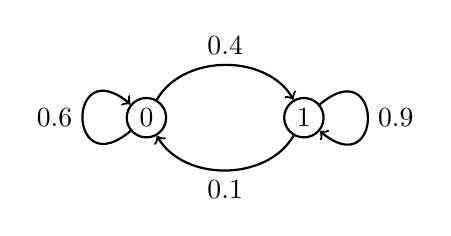
\begin{tikzpicture}
      \tikzset{punkt/.style={circle, thick, draw=black, minimum width=0.5cm,inner sep=0}}
      \node[punkt] at (1, 0)  (a){$1$};
      \node[punkt] at (-1, 0) (b){$0$};

      \draw[->, thick] (a) edge[out= 40, in = 320, looseness=8] node[right]{$0.9$} (a);
      \draw[->, thick] (b) edge[bend left=60] node[above]{$0.4$} (a);
      \draw[->, thick] (b) edge[out= 220, in = 140, looseness=8] node[left]{$0.6$} (b);
      \draw[->, thick] (a) edge[bend left=60] node[below]{$0.1$} (b);
    \end{tikzpicture}
    \caption{Overgangsgraf}
    \label{fig:eksempel_stationary}
  \end{figure}\noindent
  Fra overgangsgrafen ses det, at alle udfald intra kommunikere, og Markov kæden derfor er et eksempel på en irreducibel Markov kæde. Vi ser derudover, at ligningen
  \begin{equation*}
    \pi P_{X} = \pi \begin{bmatrix}
                      0.6 & 0.4 \\ 0.1 & 0.9
                    \end{bmatrix} = \pi
  \end{equation*}
  løses af $\pi = s \begin{bmatrix} 1 & 4 \end{bmatrix}$, hvor $s \in \R$.
  Men vi har derudover at $\pi_{1} + \pi_{2} = 1$, samt $\pi_{1}, \pi_{2} \geq 0$, da der er tale om en fordeling.
  Det følger derfor at $\pi = \begin{bmatrix} 0.2 & 0.8 \end{bmatrix}$.
\end{example}
